
%% bare_conf.tex
%% V1.3
%% 2007/01/11
%% by Michael Shell
%% See:
%% http://www.michaelshell.org/
%% for current contact information.
%%
%% This is a skeleton file demonstrating the use of IEEEtran.cls
%% (requires IEEEtran.cls version 1.7 or later) with an IEEE conference paper.
%%
%% Support sites:
%% http://www.michaelshell.org/tex/ieeetran/
%% http://www.ctan.org/tex-archive/macros/latex/contrib/IEEEtran/
%% and
%% http://www.ieee.org/

%%*************************************************************************
%% Legal Notice:
%% This code is offered as-is without any warranty either expressed or
%% implied; without even the implied warranty of MERCHANTABILITY or
%% FITNESS FOR A PARTICULAR PURPOSE! 
%% User assumes all risk.
%% In no event shall IEEE or any contributor to this code be liable for
%% any damages or losses, including, but not limited to, incidental,
%% consequential, or any other damages, resulting from the use or misuse
%% of any information contained here.
%%
%% All comments are the opinions of their respective authors and are not
%% necessarily endorsed by the IEEE.
%%
%% This work is distributed under the LaTeX Project Public License (LPPL)
%% ( http://www.latex-project.org/ ) version 1.3, and may be freely used,
%% distributed and modified. A copy of the LPPL, version 1.3, is included
%% in the base LaTeX documentation of all distributions of LaTeX released
%% 2003/12/01 or later.
%% Retain all contribution notices and credits.
%% ** Modified files should be clearly indicated as such, including  **
%% ** renaming them and changing author support contact information. **
%%
%% File list of work: IEEEtran.cls, IEEEtran_HOWTO.pdf, bare_adv.tex,
%%                    bare_conf.tex, bare_jrnl.tex, bare_jrnl_compsoc.tex
%%*************************************************************************

% *** Authors should verify (and, if needed, correct) their LaTeX system  ***
% *** with the testflow diagnostic prior to trusting their LaTeX platform ***
% *** with production work. IEEE's font choices can trigger bugs that do  ***
% *** not appear when using other class files.                            ***
% The testflow support page is at:
% http://www.michaelshell.org/tex/testflow/



% Note that the a4paper option is mainly intended so that authors in
% countries using A4 can easily print to A4 and see how their papers will
% look in print - the typesetting of the document will not typically be
% affected with changes in paper size (but the bottom and side margins will).
% Use the testflow package mentioned above to verify correct handling of
% both paper sizes by the user's LaTeX system.
%
% Also note that the "draftcls" or "draftclsnofoot", not "draft", option
% should be used if it is desired that the figures are to be displayed in
% draft mode.
%
\documentclass[conference]{IEEEtran}
% Add the compsoc option for Computer Society conferences.
%
% If IEEEtran.cls has not been installed into the LaTeX system files,
% manually specify the path to it like:
% \documentclass[conference]{../sty/IEEEtran}





% Some very useful LaTeX packages include:
% (uncomment the ones you want to load)


% *** MISC UTILITY PACKAGES ***
%
%\usepackage{ifpdf}
% Heiko Oberdiek's ifpdf.sty is very useful if you need conditional
% compilation based on whether the output is pdf or dvi.
% usage:
% \ifpdf
%   % pdf code
% \else
%   % dvi code
% \fi
% The latest version of ifpdf.sty can be obtained from:
% http://www.ctan.org/tex-archive/macros/latex/contrib/oberdiek/
% Also, note that IEEEtran.cls V1.7 and later provides a builtin
% \ifCLASSINFOpdf conditional that works the same way.
% When switching from latex to pdflatex and vice-versa, the compiler may
% have to be run twice to clear warning/error messages.






% *** CITATION PACKAGES ***
%
%\usepackage{cite}
% cite.sty was written by Donald Arseneau
% V1.6 and later of IEEEtran pre-defines the format of the cite.sty package
% \cite{} output to follow that of IEEE. Loading the cite package will
% result in citation numbers being automatically sorted and properly
% "compressed/ranged". e.g., [1], [9], [2], [7], [5], [6] without using
% cite.sty will become [1], [2], [5]--[7], [9] using cite.sty. cite.sty's
% \cite will automatically add leading space, if needed. Use cite.sty's
% noadjust option (cite.sty V3.8 and later) if you want to turn this off.
% cite.sty is already installed on most LaTeX systems. Be sure and use
% version 4.0 (2003-05-27) and later if using hyperref.sty. cite.sty does
% not currently provide for hyperlinked citations.
% The latest version can be obtained at:
% http://www.ctan.org/tex-archive/macros/latex/contrib/cite/
% The documentation is contained in the cite.sty file itself.






% *** GRAPHICS RELATED PACKAGES ***
%
\ifCLASSINFOpdf
  % \usepackage[pdftex]{graphicx}
  % declare the path(s) where your graphic files are
  % \graphicspath{{../pdf/}{../jpeg/}}
  % and their extensions so you won't have to specify these with
  % every instance of \includegraphics
  % \DeclareGraphicsExtensions{.pdf,.jpeg,.png}
\else
  % or other class option (dvipsone, dvipdf, if not using dvips). graphicx
  % will default to the driver specified in the system graphics.cfg if no
  % driver is specified.
  % \usepackage[dvips]{graphicx}
  % declare the path(s) where your graphic files are
  % \graphicspath{{../eps/}}
  % and their extensions so you won't have to specify these with
  % every instance of \includegraphics
  % \DeclareGraphicsExtensions{.eps}
\fi
% graphicx was written by David Carlisle and Sebastian Rahtz. It is
% required if you want graphics, photos, etc. graphicx.sty is already
% installed on most LaTeX systems. The latest version and documentation can
% be obtained at: 
% http://www.ctan.org/tex-archive/macros/latex/required/graphics/
% Another good source of documentation is "Using Imported Graphics in
% LaTeX2e" by Keith Reckdahl which can be found as epslatex.ps or
% epslatex.pdf at: http://www.ctan.org/tex-archive/info/
%
% latex, and pdflatex in dvi mode, support graphics in encapsulated
% postscript (.eps) format. pdflatex in pdf mode supports graphics
% in .pdf, .jpeg, .png and .mps (metapost) formats. Users should ensure
% that all non-photo figures use a vector format (.eps, .pdf, .mps) and
% not a bitmapped formats (.jpeg, .png). IEEE frowns on bitmapped formats
% which can result in "jaggedy"/blurry rendering of lines and letters as
% well as large increases in file sizes.
%
% You can find documentation about the pdfTeX application at:
% http://www.tug.org/applications/pdftex





% *** MATH PACKAGES ***
%
%\usepackage[cmex10]{amsmath}
% A popular package from the American Mathematical Society that provides
% many useful and powerful commands for dealing with mathematics. If using
% it, be sure to load this package with the cmex10 option to ensure that
% only type 1 fonts will utilized at all point sizes. Without this option,
% it is possible that some math symbols, particularly those within
% footnotes, will be rendered in bitmap form which will result in a
% document that can not be IEEE Xplore compliant!
%
% Also, note that the amsmath package sets \interdisplaylinepenalty to 10000
% thus preventing page breaks from occurring within multiline equations. Use:
%\interdisplaylinepenalty=2500
% after loading amsmath to restore such page breaks as IEEEtran.cls normally
% does. amsmath.sty is already installed on most LaTeX systems. The latest
% version and documentation can be obtained at:
% http://www.ctan.org/tex-archive/macros/latex/required/amslatex/math/





% *** SPECIALIZED LIST PACKAGES ***
%
%\usepackage{algorithmic}
% algorithmic.sty was written by Peter Williams and Rogerio Brito.
% This package provides an algorithmic environment fo describing algorithms.
% You can use the algorithmic environment in-text or within a figure
% environment to provide for a floating algorithm. Do NOT use the algorithm
% floating environment provided by algorithm.sty (by the same authors) or
% algorithm2e.sty (by Christophe Fiorio) as IEEE does not use dedicated
% algorithm float types and packages that provide these will not provide
% correct IEEE style captions. The latest version and documentation of
% algorithmic.sty can be obtained at:
% http://www.ctan.org/tex-archive/macros/latex/contrib/algorithms/
% There is also a support site at:
% http://algorithms.berlios.de/index.html
% Also of interest may be the (relatively newer and more customizable)
% algorithmicx.sty package by Szasz Janos:
% http://www.ctan.org/tex-archive/macros/latex/contrib/algorithmicx/




% *** ALIGNMENT PACKAGES ***
%
%\usepackage{array}
% Frank Mittelbach's and David Carlisle's array.sty patches and improves
% the standard LaTeX2e array and tabular environments to provide better
% appearance and additional user controls. As the default LaTeX2e table
% generation code is lacking to the point of almost being broken with
% respect to the quality of the end results, all users are strongly
% advised to use an enhanced (at the very least that provided by array.sty)
% set of table tools. array.sty is already installed on most systems. The
% latest version and documentation can be obtained at:
% http://www.ctan.org/tex-archive/macros/latex/required/tools/


%\usepackage{mdwmath}
%\usepackage{mdwtab}
% Also highly recommended is Mark Wooding's extremely powerful MDW tools,
% especially mdwmath.sty and mdwtab.sty which are used to format equations
% and tables, respectively. The MDWtools set is already installed on most
% LaTeX systems. The lastest version and documentation is available at:
% http://www.ctan.org/tex-archive/macros/latex/contrib/mdwtools/


% IEEEtran contains the IEEEeqnarray family of commands that can be used to
% generate multiline equations as well as matrices, tables, etc., of high
% quality.


%\usepackage{eqparbox}
% Also of notable interest is Scott Pakin's eqparbox package for creating
% (automatically sized) equal width boxes - aka "natural width parboxes".
% Available at:
% http://www.ctan.org/tex-archive/macros/latex/contrib/eqparbox/





% *** SUBFIGURE PACKAGES ***
%\usepackage[tight,footnotesize]{subfigure}
% subfigure.sty was written by Steven Douglas Cochran. This package makes it
% easy to put subfigures in your figures. e.g., "Figure 1a and 1b". For IEEE
% work, it is a good idea to load it with the tight package option to reduce
% the amount of white space around the subfigures. subfigure.sty is already
% installed on most LaTeX systems. The latest version and documentation can
% be obtained at:
% http://www.ctan.org/tex-archive/obsolete/macros/latex/contrib/subfigure/
% subfigure.sty has been superceeded by subfig.sty.



%\usepackage[caption=false]{caption}
%\usepackage[font=footnotesize]{subfig}
% subfig.sty, also written by Steven Douglas Cochran, is the modern
% replacement for subfigure.sty. However, subfig.sty requires and
% automatically loads Axel Sommerfeldt's caption.sty which will override
% IEEEtran.cls handling of captions and this will result in nonIEEE style
% figure/table captions. To prevent this problem, be sure and preload
% caption.sty with its "caption=false" package option. This is will preserve
% IEEEtran.cls handing of captions. Version 1.3 (2005/06/28) and later 
% (recommended due to many improvements over 1.2) of subfig.sty supports
% the caption=false option directly:
%\usepackage[caption=false,font=footnotesize]{subfig}
%
% The latest version and documentation can be obtained at:
% http://www.ctan.org/tex-archive/macros/latex/contrib/subfig/
% The latest version and documentation of caption.sty can be obtained at:
% http://www.ctan.org/tex-archive/macros/latex/contrib/caption/




% *** FLOAT PACKAGES ***
%
%\usepackage{fixltx2e}
% fixltx2e, the successor to the earlier fix2col.sty, was written by
% Frank Mittelbach and David Carlisle. This package corrects a few problems
% in the LaTeX2e kernel, the most notable of which is that in current
% LaTeX2e releases, the ordering of single and double column floats is not
% guaranteed to be preserved. Thus, an unpatched LaTeX2e can allow a
% single column figure to be placed prior to an earlier double column
% figure. The latest version and documentation can be found at:
% http://www.ctan.org/tex-archive/macros/latex/base/



%\usepackage{stfloats}
% stfloats.sty was written by Sigitas Tolusis. This package gives LaTeX2e
% the ability to do double column floats at the bottom of the page as well
% as the top. (e.g., "\begin{figure*}[!b]" is not normally possible in
% LaTeX2e). It also provides a command:
%\fnbelowfloat
% to enable the placement of footnotes below bottom floats (the standard
% LaTeX2e kernel puts them above bottom floats). This is an invasive package
% which rewrites many portions of the LaTeX2e float routines. It may not work
% with other packages that modify the LaTeX2e float routines. The latest
% version and documentation can be obtained at:
% http://www.ctan.org/tex-archive/macros/latex/contrib/sttools/
% Documentation is contained in the stfloats.sty comments as well as in the
% presfull.pdf file. Do not use the stfloats baselinefloat ability as IEEE
% does not allow \baselineskip to stretch. Authors submitting work to the
% IEEE should note that IEEE rarely uses double column equations and
% that authors should try to avoid such use. Do not be tempted to use the
% cuted.sty or midfloat.sty packages (also by Sigitas Tolusis) as IEEE does
% not format its papers in such ways.





% *** PDF, URL AND HYPERLINK PACKAGES ***
%
%\usepackage{url}
% url.sty was written by Donald Arseneau. It provides better support for
% handling and breaking URLs. url.sty is already installed on most LaTeX
% systems. The latest version can be obtained at:
% http://www.ctan.org/tex-archive/macros/latex/contrib/misc/
% Read the url.sty source comments for usage information. Basically,
% \url{my_url_here}.





% *** Do not adjust lengths that control margins, column widths, etc. ***
% *** Do not use packages that alter fonts (such as pslatex).         ***
% There should be no need to do such things with IEEEtran.cls V1.6 and later.
% (Unless specifically asked to do so by the journal or conference you plan
% to submit to, of course. )
\usepackage{graphicx}
\usepackage{amsmath}
\usepackage{url}
% correct bad hyphenation here
\hyphenation{op-tical net-works semi-conduc-tor}


\begin{document}
%
% paper title
% can use linebreaks \\ within to get better formatting as desired
\title{Reliable Data Communication Over HF Link Using System On Chip Technology}


% author names and affiliations
% use a multiple column layout for up to three different
% affiliations
\author{\IEEEauthorblockN{Somkheart Kraisin}
\IEEEauthorblockA{
	Department of Research and Development  Defence \\ 
	Technology Institute Ministry of Defence \\
	Nonthaburi ,Thailand \\
	Email : somkheart.k@dti.or.th}
\and
\IEEEauthorblockN{Wichai Pawgasame}
\IEEEauthorblockA{
	Department of Research and Development  Defence \\ 
	Technology Institute Ministry of Defence \\
	Nonthaburi ,Thailand \\
	Email : wichai.p@dti.or.th}
}

% conference papers do not typically use \thanks and this command
% is locked out in conference mode. If really needed, such as for
% the acknowledgment of grants, issue a \IEEEoverridecommandlockouts
% after \documentclass

% for over three affiliations, or if they all won't fit within the width
% of the page, use this alternative format:
% 
%\author{\IEEEauthorblockN{Michael Shell\IEEEauthorrefmark{1},
%Homer Simpson\IEEEauthorrefmark{2},
%James Kirk\IEEEauthorrefmark{3}, 
%Montgomery Scott\IEEEauthorrefmark{3} and
%Eldon Tyrell\IEEEauthorrefmark{4}}
%\IEEEauthorblockA{\IEEEauthorrefmark{1}School of Electrical and Computer Engineering\\
%Georgia Institute of Technology,
%Atlanta, Georgia 30332--0250\\ Email: see http://www.michaelshell.org/contact.html}
%\IEEEauthorblockA{\IEEEauthorrefmark{2}Twentieth Century Fox, Springfield, USA\\
%Email: homer@thesimpsons.com}
%\IEEEauthorblockA{\IEEEauthorrefmark{3}Starfleet Academy, San Francisco, California 96678-2391\\
%Telephone: (800) 555--1212, Fax: (888) 555--1212}
%\IEEEauthorblockA{\IEEEauthorrefmark{4}Tyrell Inc., 123 Replicant Street, Los Angeles, California 90210--4321}}




% use for special paper notices
%\IEEEspecialpapernotice{(Invited Paper)}




% make the title area
\maketitle


\begin{abstract}
%\boldmath
HF communication is one of the important aspects in military radio communication, even though it has been seen as a difficult and tedious task because of instability of ionosphere layer. To make HF communication becomes easier, many digital techniques have been introduced. It is also desirable to have all these techniques implemented in a single radio. This can be achieved through software defined radio (SDR) concept. Thus, a HF radio becomes more like a computer whose radio functions can be implemented through software. This paper presents some of the modern digital techniques and software defined radio architecture for HF communication aspect using System-on-Chip and FPGA technologies.
\end{abstract}
% IEEEtran.cls defaults to using nonbold math in the Abstract.
% This preserves the distinction between vectors and scalars. However,
% if the conference you are submitting to favors bold math in the abstract,
% then you can use LaTeX's standard command \boldmath at the very start
% of the abstract to achieve this. Many IEEE journals/conferences frown on
% math in the abstract anyway.

% no keywords




% For peer review papers, you can put extra information on the cover
% page as needed:
% \ifCLASSOPTIONpeerreview
% \begin{center} \bfseries EDICS Category: 3-BBND \end{center}
% \fi
%
% For peerreview papers, this IEEEtran command inserts a page break and
% creates the second title. It will be ignored for other modes.
\IEEEpeerreviewmaketitle

\section{Introduction}
% no \IEEEPARstart
Our world has changed from the Industrial Age to the Information Age due to the renovation in the information technology and communications. Military concept has been affected as well. The developments in information technology and communications drive the battlefield into the new era of an Information Warfare, or Network-Centric Warfare by connecting different units and forces into the network and information system. The main components for the stability of the system are the Centric Warfare and the well-design infrastructure on the various support systems, including secured, flexible, compatible, and cost-effective communication and telecommunication equipment. Radio Centric Network integrates information from various networks, including radar, satellite, airborne and PC data; with the HF, VHF and UHF radio systems. This allows combination between control center and tactical units on the same network for the effective operations. Software defined radio (SDR) concept, especially for high frequency (HF) ManPack or small-size radio for mobile use, is one of the main technology applicable to this innovation. SDR consists of a general hardware platform and upgradable software that allow implementation of different frequencies, desired bandwidth, functions, and output power level. SDR also has the flexibility to allow new software installation without changing or replacing new hardware modules. This paper focuses on some of modern HF technologies and the exclusive design of the software defined HF radio.
\section{Background}
	\subsection{HF Chanel}
The High Frequency (HF) band is between 1.6 - 30 MHz. It is the main frequency band for maritime, military and aeronautical systems and global communication. In this band, radio waves can propagate in two paths; the ground wave propagation path and the sky wave propagation path. There are three types of ground waves, including direct wave, ground reflected wave and surface wave. The ground waves are used to communicate within near distance due to the high rate of distortion. It is often used for communication between ships and stations on the coast since surface waves can propagate over a sea surface with less attenuation. Therefore, the communication can be produced in longer distance. On the other hand, the sky wave can propagate to a remote station at longer distance by use of reflected 
The High Frequency (HF) band is between 1.6 - 30 MHz. It is the main frequency band for maritime, military and aeronautical systems and global communication. In this band, radio waves can propagate in two paths; the ground wave propagation path and the sky wave propagation path. There are three types of ground waves, including direct wave, ground reflected wave and surface wave. The ground waves are used to communicate within near distance due to the high rate of distortion. It is often used for communication between ships and stations on the coast since surface waves can propagate over a sea surface with less attenuation. Therefore, the communication can be produced in longer distance. On the other hand, the sky wave can propagate to a remote station at longer distance by use of reflected 

\begin{figure}[h!]
	\centering
	\reflectbox{%
		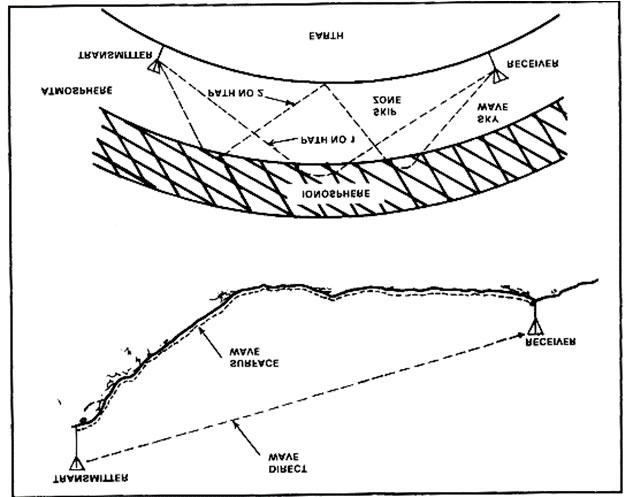
\includegraphics[width=0.5\textwidth,angle=180]{hf-1.jpg}}
	\caption{Ground Waves and Sky Waves Propagation from [1]}
\end{figure}

\subsection{Conventional HF radio}
The primary components of the HF radio system fall into three groups, which are transmitters, receivers and antennas. In many modern radio sets, the transmitter and receiver are combined into a single unit called a transceiver. The transmitter consists of the exciter, which modulates the information with the carrier signal into the signal to be transmitted. The power amplifier, then, boosts the output power of the signal before sending it through the antenna. Then, the receiver side will select a desired signal, amplify it to a suitable level, and recover the information through the process of demodulation. Figure 2-2 illustrates conventional HF radio system.
Conventional radio system establishes contact or connections by tuning to the appropriate channel and transmits and receives messages through the particular HF frequency or channel. In conventional voice HF operations, when the radio system loses connectivity, the radio operator must search for another channel. Various products and techniques, as well as the skill and experience of the radio operator are extremely important when determining the alternate channels. Even with a highly skilled radio operator, the time spent searching for alternate channels affects the operation of the radio system since it can be as long as several minutes. Thus, there is a need for a radio system that reduces search time associated with selecting alternate channels, an automatic algorithm that can automatically select a channel for HF operations, and a channel selection algorithm that does not affect communication on the other channels.

\begin{figure}[h!]
	\centering
	\reflectbox{%
		
		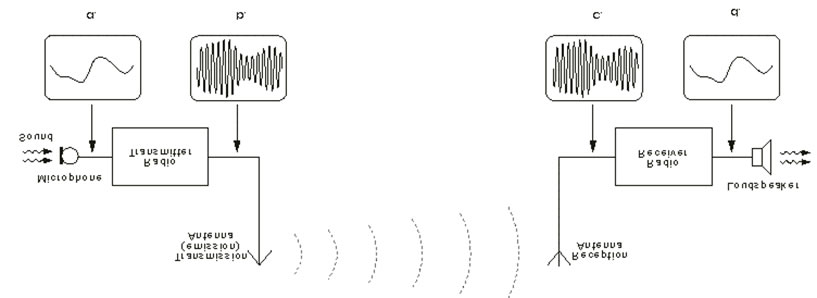
\includegraphics[width=0.5\textwidth,angle=180]{hf-2.jpg}}
	\caption{Conventional HF Radio Transmission from [2]}
\end{figure}

\section{Modern HF technologies}
An old analog military HF radio was suffers from unpredictable sky wave channel through ionosphere, unsecure communication, poor voice quality, and very slow data rate. As digital technologies have improved and become more popular, these problems have been solved. The conventional analog HF radio has transformed into digital HF radio with abilities to overcome unreliable HF channel and provide high data rate. In this section, the modern military HF radio technologies will be discussed.
\subsection{Cognitive HF radio}
According to [3], cognitive radio is a radio that can sense its operating environment and adapt its radio operating behavior to any changes in operating environment. Basically, cognitive radio should have the ability to adapt and learn. This can be achieved through artificial intelligence (AI) and software technologies. Hence, cognitive radio utilizes the concept of software defined radio to achieve its cognitive functions. 
According to [4], STANAG 4538 has defined an automatic radio control function called automatic link establishment (ALE) for modern military HF radios. This ability is classified as one of cognitive radio capabilities [5]. ALE is a technique that allows HF radio to select the best HF channel automatically. In ALE system, each radio station is assigned with an address in a network and a set of channels. When a radio is not operating, it will try to link with other stations in a network using assigned channels and measure signal quality in each link. This method is called link quality analysis (LQA). According to [4], these measurements will be stored in a LQA matrix as illustrated in Figure 3-1. When station 1 wants to communicate another station in a network, a radio consults with LQA matrix to select the best channel for each communication

\begin{figure}[h!]
	\centering
	\reflectbox{%
		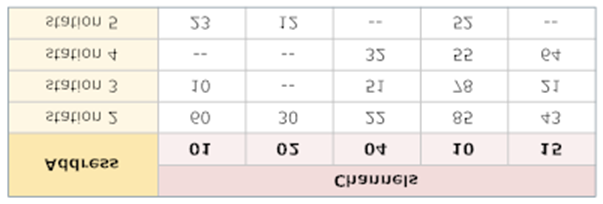
\includegraphics[width=0.5\textwidth,angle=180]{hf-3-1.png}}
	\caption{LQA matrix for station 1 according to [4]}
\end{figure}

\subsection{Data transmission}
At the very beginning, HF radios used CW modulation for data communication. CW modulation carries information by varying on-off period of carrier wave according to Morse code [6]. Data is vulnerable to noises and interferences, and data rate is very slow. As many digital modulation techniques has been developed and improved, a digital HF radio can use many digital modulation waveforms that suitable for HF channel to transmit data at higher data rate. In addition, forward error correction (FEC) coding and interleaving can be applied in HF data communication to provide reliable data. FEC adds redundancy to data while interleaving arranges data stream such that burst error has less effect on data. Voice signal can be translated into binary data stream using digital voice coder (Vocoder), hence it can take advantage of digital transmission. Figure 3-2 lists some modern waveform standards for military HF radio according to [4][7]. In modern military HF radio, it is desirable to have all these waveforms implemented in one radio. This can be achieved through software defined radio concept.
\begin{figure}[h!]
	\centering
	\reflectbox{%
		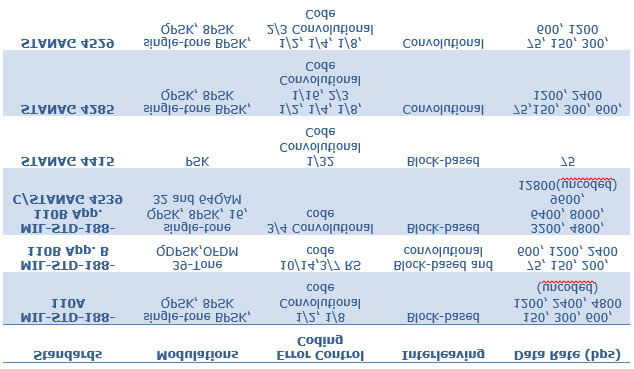
\includegraphics[width=0.5\textwidth,angle=180]{hf-3-2.jpg}}
	\caption{Modern HF waveform Standards}
\end{figure}
\subsection{Secure communication}
Secure communication is a very important aspect in military radio. There are two main processes to secure communication. One is communication security (COMSEC) where data is protected. Another is transmission security (TRANSEC) where transmission is protected. 
COMSEC on voice communication can be done using analog scrambling or cryptography. Analog scrambling technique separates signal into a number of sub-bands, then shift each sub-band into different audio sub-band and combine all sub-band together to generate one composite output signal for transmission [4].  In cryptography, voice, which is translated into binary stream by vocoder, is digitally encrypted into extremely long binary stream based on specific key and only the receiver with the same key will be able to decrypt this long binary stream. According to [4], a binary stream created in this way provides more secure than analog scrambling technique. Cryptography can be done with external device before sending to a radio for transmission. As digital technologies improved, a software defined radio can handle complex cryptography without a need for external device. Cryptography can be applied on data as well as voice.
TRANSEC applies a number of transmission techniques to prevent signal from jamming and detection. The most commonly used technique for military TRANSEC is frequency hopping [4]. In this technique, the transmitter will change transmitting frequency rapidly in a pattern only known by the receiver. This is difficult for HF channel where not all frequencies will be able to transmit. However, one study [8] shows that combining frequency hopping with link quality analysis (LQA) would make frequency hopping scheme more effective. In this study, the selection of hopping channels is made by the receiver based on LQA. This selection of hopping channels is fed back to the transmitter, so it knows what frequencies can be used for hopping. This requires a complex algorithm that can only be implemented through software.   
\section{A Software Defined HF Radio}
A modern military HF radio concept presented in section 3 can be implemented on single radio using software defined radio concept. According to [9], the term software defined radio is the use of hardware and software technologies to implement some of the radio functions through software operating on programmable processing technologies. In other word, a radio becomes more like a computer where its function can be programmed through software. The software defined radio architecture and technologies for modern military HF radio will be discussed in this section. 
\subsection{Basic Software Defined HF Radio Functions}
A software defined radio is a transceiver where its functions are provided by programmable signal processing hardware. In military communication, a software defined radio should provide encryption capability and the ability to switch between various modulation formats, and data rates in order to counter enemy’s eavesdropping and adapt to various operational conditions [10]. Figure 4-1 illustrates military software defined radio functional block diagram based on [10][11][12]. As illustrated in this figure, input, which can be voice or data at different data rates, is passed into the system as defined by man-machine interface (MMI). MMI specifies how radio interacts to user action and its function is defined by software resides in the digital signal processing unit. For voice input, voice is coded where various vocoders with different data rates are supported. Before crypto, data is called “Red” data whose information has not been protected yet. Then, Cryptography is applied on digital data stream. Output from crypto is called “Black” data whose information is protected by cryptography. Next, encrypted data will be further processed for transmission. This includes error control coding and baseband modulation. A digital signal processing unit should be able to generate many waveform standards as specified in Figure 3-2. 

\begin{figure}[h!]
	\centering
	\reflectbox{%
		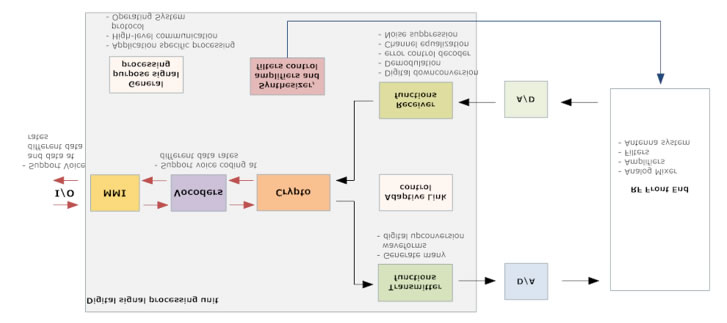
\includegraphics[width=0.5\textwidth,angle=180]{hf-4-1.jpg}}
	\caption{Modern HF waveform Standards}
\end{figure}

An adaptive link control function is used to adapt transmission characteristic to suit any changes in the channel. The modulated baseband signal is digitally up-converted to low intermediate frequency (IF) inside digital signal processing unit. Then, digital-to-analog converter (DAC) is used to convert digital IF signal to analog IF signal, and sends to RF Front End. For transmitter functions, RF Front End basically contains reconstruction filter that smooth output signal from DAC, analog mixer that converts IF signal into passband signal at carrier frequency, band-pass filters that reduces phase noise produced by local oscillator and reject unwanted signals, power amplifier (PA) that makes transmitting signal strong enough to drive an antenna, and antenna system. 
For receiver functions, RF front end should contain band-pass filters that reject unwanted signal, analog mixers that convert passband signal back to low IF signal, amplifier system controlled by automatic gain control (AGC) that maintain received signal at optimal levels, and anti-aliasing filter that reduce effect of aliasing before sampling a received signal. Analog-to-digital converter (ADC) converts analog signal to digital IF signal. Digital signal is then digitally down-converted, demodulated and error control decoded by receiver function in digital signal processing unit. In addition, this unit contains necessary functions to maintain good quality of received signal such as channel equalizer and noise rejection. Received data stream is then decrypted and decoded to information signal that is usable by the user. 
A general purpose signal processing is used for application specific data processing that requires high-level software language and complex algorithm. It is also used for implementing high-level communication protocol. It may also contain operating system for a radio. Typically, this function processes data that does not require long and complex mathematic operation. 
A synthesizer, amplifiers and filters control functions is used to control synthesizer, filters, and amplifiers in RF front end. This function includes AGC that control amplifier system to maintain low noise figure in the receiver. 
There are many up/down-conversion solutions as described in [12], the solution described in this paper is just one of many solutions for software defined HF radio. With today’s DAC and ADC technology, it is possible to directly convert digital signal in HF band into analog HF signal. In this solution [11], a digital upconverter can directly convert baseband signal into passband signal at HF frequency, and a digital downconverter can directly convert HF passband signal to baseband signal. With this solution, there is no need for external analog mixer in the RF Front End. The digital up/down-converter presented here is based on Weaver method [13] and the design is presented in [11]. Figure 4-2 and 4-3 illustrate this design

\begin{figure}[h!]
	\centering
	\reflectbox{%
		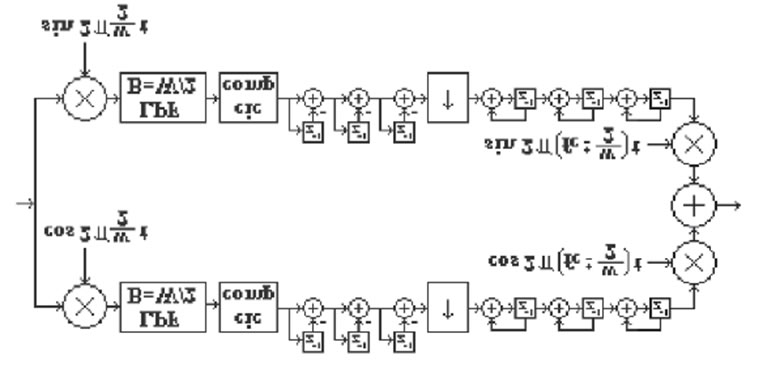
\includegraphics[width=0.5\textwidth,angle=180]{hf-4-2.jpg}}
	\caption{Weaver digital upconversion from [11]}
	\label{fig:4-2}
\end{figure}

\begin{figure}[h!]
	\centering
	\reflectbox{%
		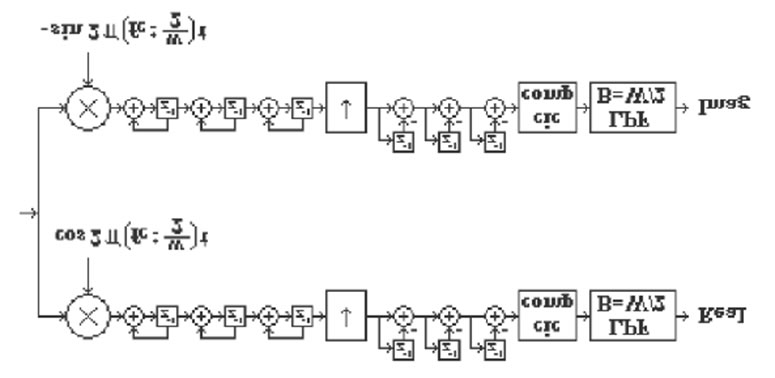
\includegraphics[width=0.5\textwidth,angle=180]{hf-4-3.jpg}}
	\caption{Weaver digital downconversion from [11]}
	\label{fig:4-3}
\end{figure}

In Weaver upconversion method, the real digital baseband signal is mixed with sinusoidal signals at the frequency equal to half bandwidth of input signal (W/2). This is to translate middle of input spectrum to be center at zero frequency. Then, liner phase low-pass filter with cutoff frequency around half bandwidth of input signal is used to filter out high frequency components. The cascaded integrator comb (CIC) filters are used to upsampling input to sample rate of 76.8 MHz [11], which is satisfied Nyquist rate for HF band (1.6 – 30 MHz). This is to guarantee that no reconstruction aliasing would occur. The output of CIC filters are then modulated with sinusoidal signals center at
\begin{figure}[h!]
	\centering
	\reflectbox{%
		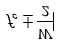
\includegraphics[width=0.1\textwidth,angle=180]{figure-math.png}}
\end{figure}
A plus sign indicates that upper side-band (USB) signal is generated, where a minus sign indicates that lower side-band (LSB) signal is generated. For Weaver downconversion method, the process is just a reverse of upconversion. The output of digital downconversion can be left as in-phase and quadrature form as illustrate in Figure 4-3. 
\subsection{Software Defined HF Radio Hardware Architecture }
According to the functional model presented in Section 4.1, a software defined HF radio would have hardware architecture as illustrated in Figure 4-4. The hardware architecture presented in this paper is based on [11][12]. This architecture is for multiband radio, which supports operation in VHF and UHF bands as well. Narrowband and wideband signal processing are also possible. For the operation in HF band, the signal can be upconverted and downconverted directly in digital signal processing unit without the use of external mixer as discussed in Section 4.1. In this section, the main components of software defined HF radio will be discussed.
\begin{figure}[h!]
	\centering
	\reflectbox{%
		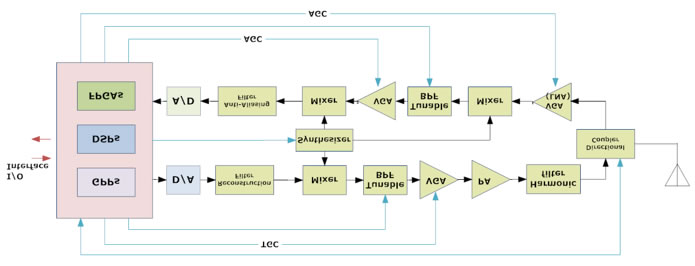
\includegraphics[width=0.5\textwidth,angle=180]{hf-4-4.jpg}}
	\caption{Weaver digital downconversion from [11]}
	\label{fig:downconversion}
\end{figure} 
\subsubsection{Digital Signal Processing unit}
The digital signal processing unit is the most important part of software defined radio. It is responsible for data and signal processing. Digital signal processing unit is based on programmable processor technologies. There are a lot of such technologies exists today. In this paper, only processor technology as described in [11] will be presented. The solution can be implemented from one of processor technologies or a combination of many processor technologies 
\subsubsection{System on Chip (SoC)}
A system on a chip or system on chip is an integrated circuit (IC) that integrates all components of a computer or other electronic system into a single chip. It may contain digital, analog, mixed-signal, and often radio-frequency functions all on a single chip 

\subsection{ADC and DAC}
The main task of DAC in software defined radio is to convert digital output signal from digital signal processing unit into analog signal. An example of DAC that is suitable for a software defined HF radio as presented in [11] is AD9744. This 14-bit DAC can support maximum rate of 210 million samples per second, which is enough to convert digital output signal from digital signal processing unit with sampling rate of 76.8 MHz.
The ADC converter converts received analog HF signal into digital signal. The solution presented in [11] is LTC2249, which can provide 14-bit 80 million samples per second with 73 dB SNR. This give a digital output signal that meet the required sampling rate for an input to the digital signal processing unit is 76.8 MHz. 
The main considerations of ADC and DAC are that they should meet required sampling rate of the input and output to the digital signal processing unit with high SNR output and less power consumption [12].
\subsection{RF Front End}
RF front end should provide analog transmitter and receiver functions. Generally, RF front end contains analog mixers, filters, and amplifiers. The hardware solution of RF front end for software defined HF radio is presented in Figure \ref{fig:downconversion}. The receiver use multi-stage IF technique such that input to the digital signal processing unit is converted to low IF signal. According to [11], analog mixer would not be needed in HF operation.
The reconstruction and anti-aliasing filters are usually the same filter. At the transmitter, it is used to smooth output from DAC and remove unwanted signal over 30 MHz HF band. At the receiver, it is used to limit input signal under 30 MHz HF band to prevent aliasing after ADC. According to [11], this filter can be implemented from 10th order Butterworth low-pass filter that allow full 30 MHz HF spectrum to pass without signal degradation. The stop-band edge is designed to attenuate signal at 38.4 MHz, which is half of output sampling rate from digital signal processing unit. The frequency response of reconstruction and anti-aliasing filter according to this solution is illustrated in Figure \ref{fig:freq_resp}.

\begin{figure}[h!]
	\centering
	\reflectbox{%
		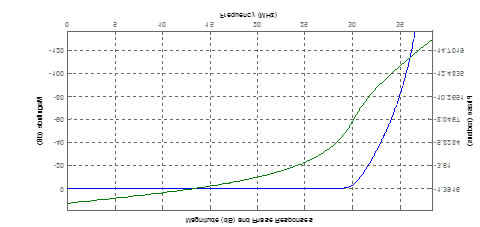
\includegraphics[width=0.5\textwidth,angle=180]{hf-4-5.jpg}}
	\caption{Frequency response of reconstruction and anti-aliasing filter}
	\label{fig:freq_resp}
\end{figure}




% An example of a floating figure using the graphicx package.
% Note that \label must occur AFTER (or within) \caption.
% For figures, \caption should occur after the \includegraphics.
% Note that IEEEtran v1.7 and later has special internal code that
% is designed to preserve the operation of \label within \caption
% even when the captionsoff option is in effect. However, because
% of issues like this, it may be the safest practice to put all your
% \label just after \caption rather than within \caption{}.
%
% Reminder: the "draftcls" or "draftclsnofoot", not "draft", class
% option should be used if it is desired that the figures are to be
% displayed while in draft mode.
%
%\begin{figure}[!t]
%\centering
%\includegraphics[width=2.5in]{myfigure}
% where an .eps filename suffix will be assumed under latex, 
% and a .pdf suffix will be assumed for pdflatex; or what has been declared
% via \DeclareGraphicsExtensions.
%\caption{Simulation Results}
%\label{fig_sim}
%\end{figure}

% Note that IEEE typically puts floats only at the top, even when this
% results in a large percentage of a column being occupied by floats.


% An example of a double column floating figure using two subfigures.
% (The subfig.sty package must be loaded for this to work.)
% The subfigure \label commands are set within each subfloat command, the
% \label for the overall figure must come after \caption.
% \hfil must be used as a separator to get equal spacing.
% The subfigure.sty package works much the same way, except \subfigure is
% used instead of \subfloat.
%
%\begin{figure*}[!t]
%\centerline{\subfloat[Case I]\includegraphics[width=2.5in]{subfigcase1}%
%\label{fig_first_case}}
%\hfil
%\subfloat[Case II]{\includegraphics[width=2.5in]{subfigcase2}%
%\label{fig_second_case}}}
%\caption{Simulation results}
%\label{fig_sim}
%\end{figure*}
%
% Note that often IEEE papers with subfigures do not employ subfigure
% captions (using the optional argument to \subfloat), but instead will
% reference/describe all of them (a), (b), etc., within the main caption.


% An example of a floating table. Note that, for IEEE style tables, the 
% \caption command should come BEFORE the table. Table text will default to
% \footnotesize as IEEE normally uses this smaller font for tables.
% The \label must come after \caption as always.
%
%\begin{table}[!t]
%% increase table row spacing, adjust to taste
%\renewcommand{\arraystretch}{1.3}
% if using array.sty, it might be a good idea to tweak the value of
% \extrarowheight as needed to properly center the text within the cells
%\caption{An Example of a Table}
%\label{table_example}
%\centering
%% Some packages, such as MDW tools, offer better commands for making tables
%% than the plain LaTeX2e tabular which is used here.
%\begin{tabular}{|c||c|}
%\hline
%One & Two\\
%\hline
%Three & Four\\
%\hline
%\end{tabular}
%\end{table}


% Note that IEEE does not put floats in the very first column - or typically
% anywhere on the first page for that matter. Also, in-text middle ("here")
% positioning is not used. Most IEEE journals/conferences use top floats
% exclusively. Note that, LaTeX2e, unlike IEEE journals/conferences, places
% footnotes above bottom floats. This can be corrected via the \fnbelowfloat
% command of the stfloats package.



\section{Conclusion}
The communication over HF channel has been seen as a difficult task. As digital communication technologies have been developed, many of these technologies are applied into HF radio. HF communication becomes easier and more effective. Hence, the concept of HF radio has changed from analog HF radio to digital HF radio which can be implemented using software defined radio concept. In military, a software defined radio should provide security communication and the ability to switch between many waveforms and adapt to any environment. The main aspects of software defined radio architecture are digital signal processing, DAC/ADC, and RF Front End technologies. The software defined radio architecture presented in this paper is one the solutions that is suitable for HF communication. 


% conference papers do not normally have an appendix


% use section* for acknowledgement
\section*{Acknowledgment}
This work was supported in part of Basic Research
Program from Research and Development Department by the
Defence Technology Institute (Public Organization),Thailand.


% trigger a \newpage just before the given reference
% number - used to balance the columns on the last page
% adjust value as needed - may need to be readjusted if
% the document is modified later
%\IEEEtriggeratref{8}
% The "triggered" command can be changed if desired:
%\IEEEtriggercmd{\enlargethispage{-5in}}

% references section

% can use a bibliography generated by BibTeX as a .bbl file
% BibTeX documentation can be easily obtained at:
% http://www.ctan.org/tex-archive/biblio/bibtex/contrib/doc/
% The IEEEtran BibTeX style support page is at:
% http://www.michaelshell.org/tex/ieeetran/bibtex/
%\bibliographystyle{IEEEtran}
% argument is your BibTeX string definitions and bibliography database(s)
%\bibliography{IEEEabrv,../bib/paper}
%
% <OR> manually copy in the resultant .bbl file
% set second argument of \begin to the number of references
% (used to reserve space for the reference number labels box)
\begin{thebibliography}{1}

\bibitem
GlobalSecurity.Org,“FM 24-19: Chapter 3 - Antennas”, [Online]. Available: http://www.globalsecurity.org/military/library/policy/army/fm/24-19/Ch3.htm [Accessed: May 2010].

\bibitem
World Technical,“Principles of Radio Transmission”, [Online]. Available: 
http://worldtechnical.blogspot.com/2008\_12\_01\_archive.html [Accessed: May 2010]. 
\bibitem
SDR forum, “Defining Cognitive Radio and Dynamic Spectrum Access”, [Online]. Available: http://www.wirelessinnovation.org/page/Defining\_CR\_and\_DSA   [Access: May 2010].
\bibitem
RF Communications Division, Harris Corporation (2005), “Radio Communications in the Digital Age, Volume One: HF Technology, Edition 2”, 2nd Edition, October 2005, USA: Harris Corporation.
\bibitem
B.Fette, “Cognitive Radio Technology”, 2nd Edition, Academic Press, Elsevier Inc., Massachusetts, 2009.
\bibitem
Wikipedia contributors, “Continuous Wave Modulation” [Online]. Available: http://en.wikipedia.org/wiki/Continuous\_wave [Accessed: May 2010]. 
\bibitem
HOKA Electronics, “Modern Waveforms” [Online]. Available: http://www.hoka.com/tech\_info/modern\_waveforms.htm [Accessed: May 2010].
\bibitem
J.Zander, G.Malmgren, “Adaptive Frequency Hopping in HF Communications”, IEE Proc. Communication, vol. 142, pp. 99-105, April 1995. 

\bibitem
SDR forum, “Introduction to Software Defined Radio”, [Online]. Available: http://www.wirelessinnovation.org/page/Introduction\_to\_SDR  [Access: May 2010].

\bibitem
R.I.Lackey,D.W.Upmal, “Speakeasy: The Military Software Radio”, IEEE Communication Magazine, vol. 33, pp. 56-61, May 1995.  

\bibitem
M.W.Chamberlain, “A Software defined HF Radio”, IEEE MILCOM. 2005, vol. 4, pp. 2448-2453, 17-20 October 2005 

\bibitem
P.B.Kenington, “RF and Baseband Techniques for Software Defined Radio”, Artech House Mobile Commnication Series, Artech House Inc., Massachusetts, 2005.

\bibitem
D.Weaver, “A Third Method of Generation and Detection of Single-Sideband Signals”, IRE Proc., vol. 44, pp. 1703-1705, December 1956.


\bibitem
Wikipedia contributors, “Preprocessor” [Online]. Available: http://en.wikipedia.org/wiki/Preprocessor\#General\_purpose\_preprocessor   [Accessed: May 2010].

  
\end{thebibliography}



% that's all folks
\end{document}


